\makeatletter
\tikzset{
        database/.style={
            path picture={
                \draw (0, 1.5*\database@segmentheight) circle [x radius=\database@radius,y radius=\database@aspectratio*\database@radius];
                \draw (-\database@radius, 0.5*\database@segmentheight) arc [start angle=180,end angle=360,x radius=\database@radius, y radius=\database@aspectratio*\database@radius];
                \draw (-\database@radius,-0.5*\database@segmentheight) arc [start angle=180,end angle=360,x radius=\database@radius, y radius=\database@aspectratio*\database@radius];
                \draw (-\database@radius,1.5*\database@segmentheight) -- ++(0,-3*\database@segmentheight) arc [start angle=180,end angle=360,x radius=\database@radius, y radius=\database@aspectratio*\database@radius] -- ++(0,3*\database@segmentheight);
            },
            minimum width=2*\database@radius + \pgflinewidth,
            minimum height=3*\database@segmentheight + 2*\database@aspectratio*\database@radius + \pgflinewidth,
        },
        database segment height/.store in=\database@segmentheight,
        database radius/.store in=\database@radius,
        database aspect ratio/.store in=\database@aspectratio,
        database segment height=0.1cm,
        database radius=0.25cm,
        database aspect ratio=0.35,
    }
\makeatother

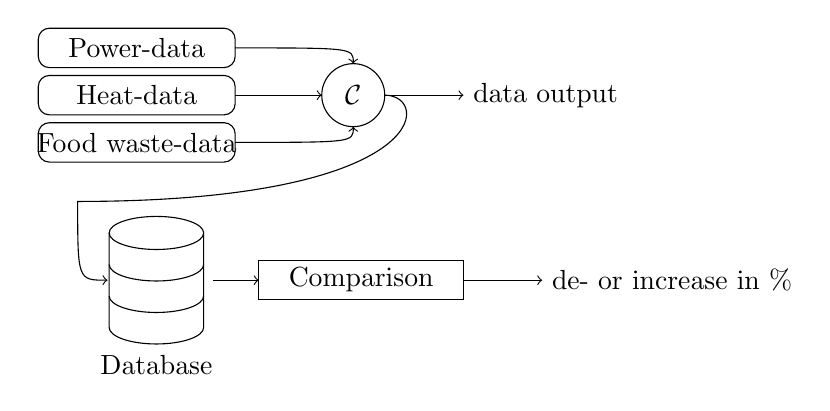
\begin{tikzpicture}
    
    %data nodes
    \draw[rounded corners] (0,2) rectangle (2.5,2.5) node[midway] {Food waste-data};
    \draw[rounded corners] (0,2.6) rectangle (2.5,3.1) node[midway] {Heat-data};
    \draw[rounded corners] (0,3.2) rectangle (2.5,3.7) node[midway] {Power-data};
    %data-proces
    \draw (4,2.85) circle (0.4) node[] {$\mathcal{C}$};
    %pile til data proces
    \draw[->] (2.5,2.25) .. controls (4,2.25) .. (4,2.45);
    \draw[->] (2.5,2.85) -- (3.6,2.85);
    \draw[->] (2.5,3.45) .. controls (4,3.45) .. (4,3.25);
    \draw[->] (4.4,2.85) -- (5.4,2.85) node[right] {data output};
    %pile til database
    \draw[->] (4.4,2.85) .. controls (5,2.85) and (5,1.5) .. (0.5,1.5) .. controls (0.5,0.5)  .. (0.88,0.5);
    %database
    \node[database,label=below:Database,database radius=0.6cm,database segment height=0.4cm] at (1.5,0.5) {};
    %pile til venstre får databasen
    \draw[->] (2.22,0.5) -- (2.8,0.5);
    %predisktiv model
    \draw (2.8,0.25) rectangle (5.4,0.75) node[midway] {Comparison};
    %pil fr apredictive model
    \draw[->] (5.4,0.5) -- (6.4,0.5) node[right] {de- or increase in \%};
    
\end{tikzpicture}